\documentclass[11pt]{article}

\usepackage{graphicx, epsfig}
\usepackage{amsmath, amssymb, latexsym}
\usepackage[english]{babel}
\usepackage{amssymb}   
%\usepackage{graphicx}
%\usepackage{float} 






% Make a larger page (shrink the margins)
%
\setlength{\textwidth}{6.7in}
\setlength{\textheight}{9.0in}
\setlength{\evensidemargin}{0.0in}
\setlength{\oddsidemargin}{0.0in}
\topmargin -0.5in
\footskip 0.5in



\title{Weekly Report for July 5th}
\author{Eric Davis}
\begin{document}
\maketitle
\medskip



\section{The Sites}
\hspace{0.5cm}

So this week I started looking at the other sites data to be able to pinpoint and compare the imaging systems between them. The issue, however, is that what I thought was a fairly robust code is not handling the other sites data very well as seen in figure 1. Most of my week was spent trying to get a working code. I do have a couple ideas I think should be able to get it working. 

\begin{figure}[h!]
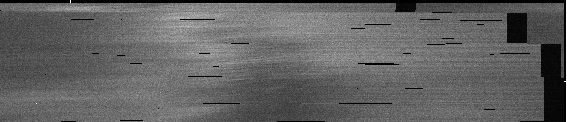
\includegraphics[scale=1.2]{bad_data.jpg}
\caption{This data is from the Gillam Manitoba sight. As seen the camera skips steps sporadically, with the black lines indicating missing data. I should hopefully have a code that can handle files like this or any other data issues by the end of Monday.}
\end{figure}



\section{Future Considerations}

I plan to continue with the goals outlined in the "Different Site Outline" document. I am still on schedule and will keep you informed if I have any issues I could use help with.

\end{document}
\end{article}